\documentclass[border=12pt]{standalone}
\usepackage{tikz}
\usepackage{amsmath,amssymb}
\usetikzlibrary{arrows.meta,positioning,shapes.geometric,fit,calc,backgrounds}

\begin{document}
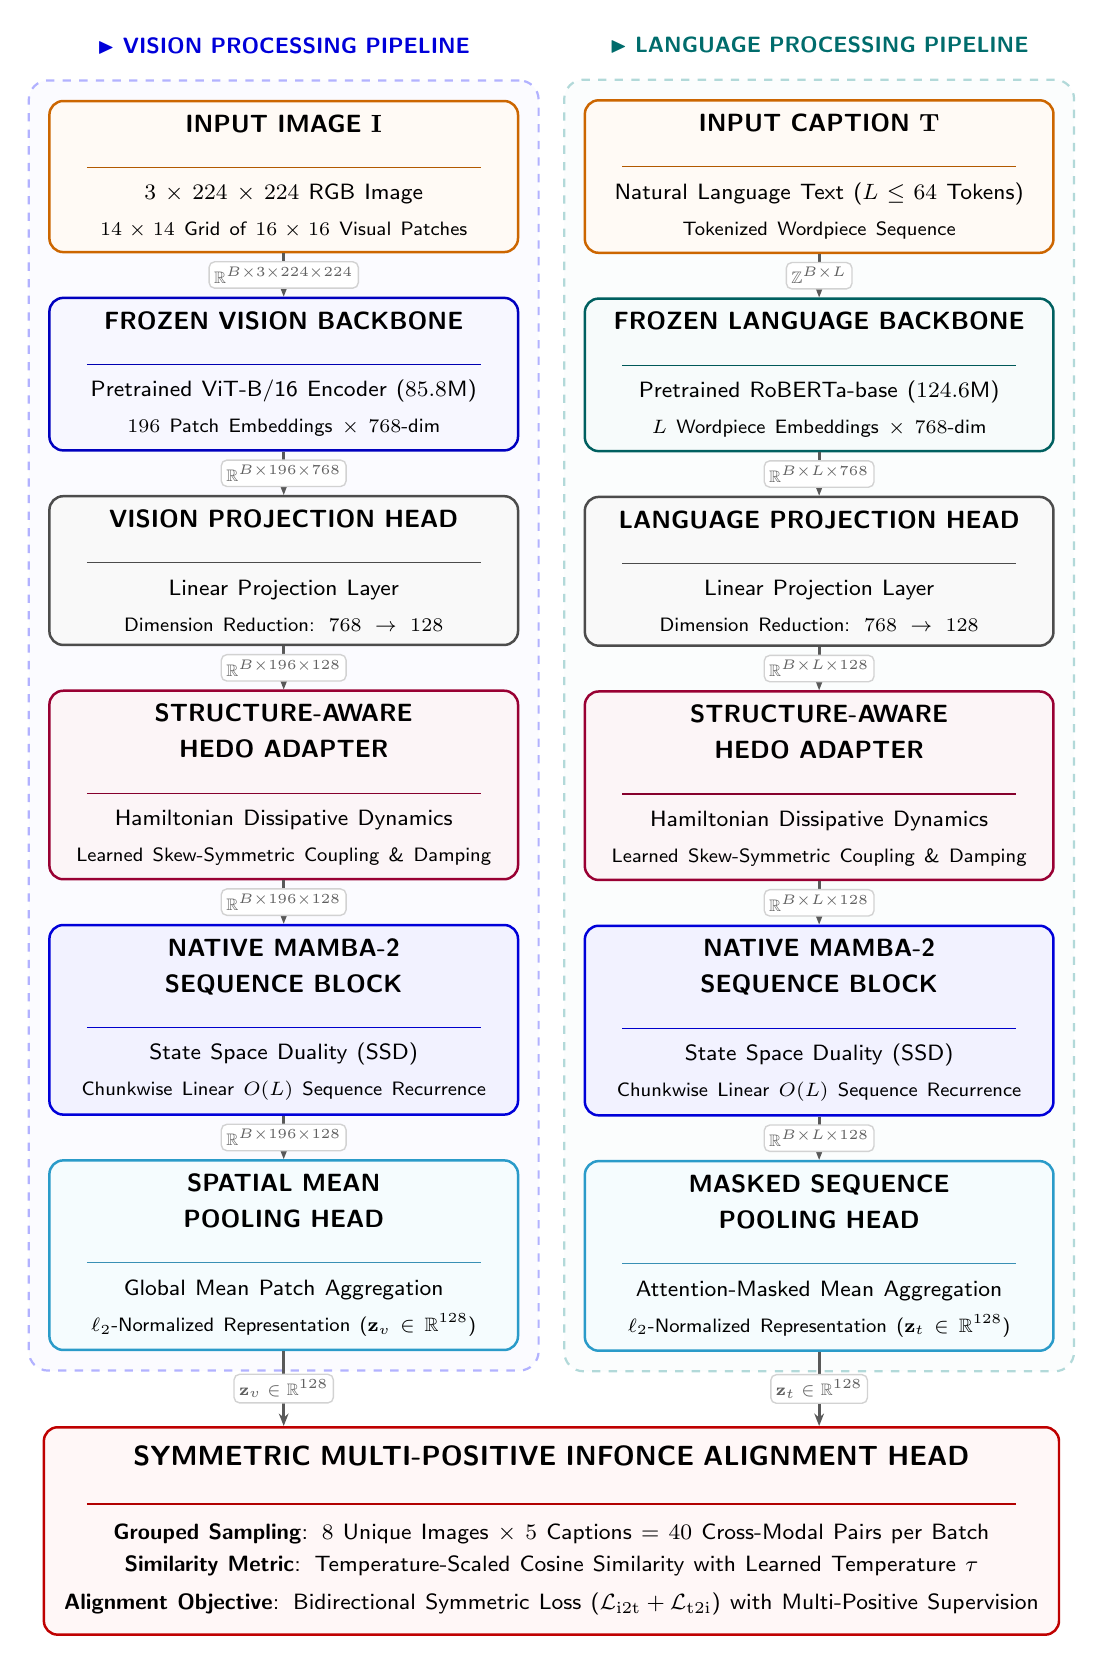
\begin{tikzpicture}[
    font=\sffamily,
    >=stealth,
    card/.style={
        draw, 
        rounded corners=5pt, 
        line width=0.9pt,
        align=center, 
        fill=white, 
        inner sep=5pt,
        text width=5.6cm,
        minimum height=1.35cm
    },
    inputcard/.style={
        card,
        draw=orange!80!black,
        fill=orange!4
    },
    visioncard/.style={
        card,
        draw=blue!75!black,
        fill=blue!3
    },
    langcard/.style={
        card,
        draw=teal!75!black,
        fill=teal!3
    },
    projcard/.style={
        card,
        draw=gray!60!black,
        fill=gray!5
    },
    hedocard/.style={
        card,
        draw=purple!80!black,
        fill=purple!4
    },
    mambacard/.style={
        card,
        draw=blue!85!black,
        fill=blue!5
    },
    poolcard/.style={
        card,
        draw=cyan!80!black,
        fill=cyan!4
    },
    losscard/.style={
        card,
        draw=red!75!black,
        fill=red!3,
        text width=12.4cm,
        inner sep=7pt
    },
    arrow/.style={
        ->,
        line width=1.0pt,
        draw=gray!70!black,
        >={Stealth[length=4.5pt, width=3.5pt]}
    },
    dimtag/.style={
        fill=white,
        draw=gray!35,
        line width=0.5pt,
        rounded corners=2pt,
        inner sep=1.8pt,
        font=\fontsize{6}{7}\selectfont\sffamily\bfseries,
        text=gray!75!black
    }
]

% ==================== VISION STREAM (LEFT COLUMN, x=3.2) ====================
\node[inputcard] (img_in) at (3.2, 9.0) {
    \textbf{\small INPUT IMAGE $\mathbf{I}$}\\[1pt]
    {\color{orange!70!black}\rule{5.0cm}{0.4pt}}\\[2pt]
    \footnotesize $3 \times 224 \times 224$ RGB Image\\[1pt]
    \scriptsize $14 \times 14$ Grid of $16 \times 16$ Visual Patches
};

\node[visioncard, below=0.55cm of img_in.south, anchor=north] (vit) {
    \textbf{\small FROZEN VISION BACKBONE}\\[1pt]
    {\color{blue!70!black}\rule{5.0cm}{0.4pt}}\\[2pt]
    \footnotesize Pretrained ViT-B/16 Encoder ($85.8\text{M}$)\\[1pt]
    \scriptsize $196$ Patch Embeddings $\times$ $768$-dim
};

\node[projcard, below=0.55cm of vit.south, anchor=north] (proj_v) {
    \textbf{\small VISION PROJECTION HEAD}\\[1pt]
    {\color{gray!60!black}\rule{5.0cm}{0.4pt}}\\[2pt]
    \footnotesize Linear Projection Layer\\[1pt]
    \scriptsize Dimension Reduction: $768 \to 128$
};

\node[hedocard, below=0.55cm of proj_v.south, anchor=north] (hedo_v) {
    \textbf{\small STRUCTURE-AWARE}\\[1pt]
    \textbf{\small HEDO ADAPTER}\\[1pt]
    {\color{purple!70!black}\rule{5.0cm}{0.4pt}}\\[2pt]
    \footnotesize Hamiltonian Dissipative Dynamics\\[1pt]
    \scriptsize Learned Skew-Symmetric Coupling \& Damping
};

\node[mambacard, below=0.55cm of hedo_v.south, anchor=north] (mamba_v) {
    \textbf{\small NATIVE MAMBA-2}\\[1pt]
    \textbf{\small SEQUENCE BLOCK}\\[1pt]
    {\color{blue!80!black}\rule{5.0cm}{0.4pt}}\\[2pt]
    \footnotesize State Space Duality (SSD)\\[1pt]
    \scriptsize Chunkwise Linear $O(L)$ Sequence Recurrence
};

\node[poolcard, below=0.55cm of mamba_v.south, anchor=north] (pool_v) {
    \textbf{\small SPATIAL MEAN}\\[1pt]
    \textbf{\small POOLING HEAD}\\[1pt]
    {\color{cyan!70!black}\rule{5.0cm}{0.4pt}}\\[2pt]
    \footnotesize Global Mean Patch Aggregation\\[1pt]
    \scriptsize $\ell_2$-Normalized Representation ($\mathbf{z}_v \in \mathbb{R}^{128}$)
};

% ==================== LANGUAGE STREAM (RIGHT COLUMN, x=10.0) ====================
\node[inputcard] (txt_in) at (10.0, 9.0) {
    \textbf{\small INPUT CAPTION $\mathbf{T}$}\\[1pt]
    {\color{orange!70!black}\rule{5.0cm}{0.4pt}}\\[2pt]
    \footnotesize Natural Language Text ($L \le 64$ Tokens)\\[1pt]
    \scriptsize Tokenized Wordpiece Sequence
};

\node[langcard, below=0.55cm of txt_in.south, anchor=north] (roberta) {
    \textbf{\small FROZEN LANGUAGE BACKBONE}\\[1pt]
    {\color{teal!70!black}\rule{5.0cm}{0.4pt}}\\[2pt]
    \footnotesize Pretrained RoBERTa-base ($124.6\text{M}$)\\[1pt]
    \scriptsize $L$ Wordpiece Embeddings $\times$ $768$-dim
};

\node[projcard, below=0.55cm of roberta.south, anchor=north] (proj_t) {
    \textbf{\small LANGUAGE PROJECTION HEAD}\\[1pt]
    {\color{gray!60!black}\rule{5.0cm}{0.4pt}}\\[2pt]
    \footnotesize Linear Projection Layer\\[1pt]
    \scriptsize Dimension Reduction: $768 \to 128$
};

\node[hedocard, below=0.55cm of proj_t.south, anchor=north] (hedo_t) {
    \textbf{\small STRUCTURE-AWARE}\\[1pt]
    \textbf{\small HEDO ADAPTER}\\[1pt]
    {\color{purple!70!black}\rule{5.0cm}{0.4pt}}\\[2pt]
    \footnotesize Hamiltonian Dissipative Dynamics\\[1pt]
    \scriptsize Learned Skew-Symmetric Coupling \& Damping
};

\node[mambacard, below=0.55cm of hedo_t.south, anchor=north] (mamba_t) {
    \textbf{\small NATIVE MAMBA-2}\\[1pt]
    \textbf{\small SEQUENCE BLOCK}\\[1pt]
    {\color{blue!80!black}\rule{5.0cm}{0.4pt}}\\[2pt]
    \footnotesize State Space Duality (SSD)\\[1pt]
    \scriptsize Chunkwise Linear $O(L)$ Sequence Recurrence
};

\node[poolcard, below=0.55cm of mamba_t.south, anchor=north] (pool_t) {
    \textbf{\small MASKED SEQUENCE}\\[1pt]
    \textbf{\small POOLING HEAD}\\[1pt]
    {\color{cyan!70!black}\rule{5.0cm}{0.4pt}}\\[2pt]
    \footnotesize Attention-Masked Mean Aggregation\\[1pt]
    \scriptsize $\ell_2$-Normalized Representation ($\mathbf{z}_t \in \mathbb{R}^{128}$)
};

% ==================== ALIGNMENT HEAD (BOTTOM, centered at x=6.6) ====================
\node[losscard, below=0.95cm of pool_v.south, anchor=north, xshift=3.4cm] (infonce) {
    \textbf{\normalsize SYMMETRIC MULTI-POSITIVE INFONCE ALIGNMENT HEAD}\\[2pt]
    {\color{red!70!black}\rule{11.8cm}{0.5pt}}\\[3pt]
    \footnotesize \textbf{Grouped Sampling}: $8$ Unique Images $\times$ $5$ Captions = $40$ Cross-Modal Pairs per Batch\\[2pt]
    \footnotesize \textbf{Similarity Metric}: Temperature-Scaled Cosine Similarity with Learned Temperature $\tau$\\[2pt]
    \footnotesize \textbf{Alignment Objective}: Bidirectional Symmetric Loss ($\mathcal{L}_{\mathrm{i2t}} + \mathcal{L}_{\mathrm{t2i}}$) with Multi-Positive Supervision
};

% ==================== ARROWS WITH TENSOR DIMENSIONS ====================
% Vision Stream Arrows
\draw[arrow] (img_in) -- (vit) 
    node[midway, dimtag] {$\mathbb{R}^{B \times 3 \times 224 \times 224}$};
\draw[arrow] (vit) -- (proj_v) 
    node[midway, dimtag] {$\mathbb{R}^{B \times 196 \times 768}$};
\draw[arrow] (proj_v) -- (hedo_v) 
    node[midway, dimtag] {$\mathbb{R}^{B \times 196 \times 128}$};
\draw[arrow] (hedo_v) -- (mamba_v) 
    node[midway, dimtag] {$\mathbb{R}^{B \times 196 \times 128}$};
\draw[arrow] (mamba_v) -- (pool_v) 
    node[midway, dimtag] {$\mathbb{R}^{B \times 196 \times 128}$};
\draw[arrow] (pool_v.south) -- (pool_v.south |- infonce.north) 
    node[midway, dimtag] {$\mathbf{z}_v \in \mathbb{R}^{128}$};

% Language Stream Arrows
\draw[arrow] (txt_in) -- (roberta) 
    node[midway, dimtag] {$\mathbb{Z}^{B \times L}$};
\draw[arrow] (roberta) -- (proj_t) 
    node[midway, dimtag] {$\mathbb{R}^{B \times L \times 768}$};
\draw[arrow] (proj_t) -- (hedo_t) 
    node[midway, dimtag] {$\mathbb{R}^{B \times L \times 128}$};
\draw[arrow] (hedo_t) -- (mamba_t) 
    node[midway, dimtag] {$\mathbb{R}^{B \times L \times 128}$};
\draw[arrow] (mamba_t) -- (pool_t) 
    node[midway, dimtag] {$\mathbb{R}^{B \times L \times 128}$};
\draw[arrow] (pool_t.south) -- (pool_t.south |- infonce.north) 
    node[midway, dimtag] {$\mathbf{z}_t \in \mathbb{R}^{128}$};

% ==================== BACKGROUND STREAM CONTAINERS ====================
\begin{scope}[on background layer]
    \node[draw=blue!30, fill=blue!1.5, dashed, rounded corners=7pt, line width=0.8pt, 
          fit=(img_in)(pool_v), inner xsep=7pt, inner ysep=7pt] (vision_container) {};
    \node[draw=teal!30, fill=teal!1.5, dashed, rounded corners=7pt, line width=0.8pt, 
          fit=(txt_in)(pool_t), inner xsep=7pt, inner ysep=7pt] (lang_container) {};
\end{scope}

% Stream Header Labels
\node[above=0.20cm of vision_container.north, font=\sffamily\bfseries\footnotesize, text=blue!85!black] {
    $\blacktriangleright$ VISION PROCESSING PIPELINE
};
\node[above=0.20cm of lang_container.north, font=\sffamily\bfseries\footnotesize, text=teal!85!black] {
    $\blacktriangleright$ LANGUAGE PROCESSING PIPELINE
};

\end{tikzpicture}
\end{document}
